\section{数据预处理与探索性分析}
\subsection{数据结构与处理原则}
数据集包含1904条记录和7个字段，分别为药物名称、溶剂名称、药物SMILES、溶剂SMILES、温度、溶解度对数及溶解度单位。目标记为$y=\mathrm{Solubility\_log10}$，浓度显示采用$10^y$，其单位按数据表中的mol/L解释。温度按数据集数值尺度建模和绘图，原表未标注单位。

全量结构检查得到168种药物结构、49种溶剂结构及646种精确药物--溶剂组合。全部SMILES可解析，模型输入字段未发现缺失值。药物名称共有186种，其中17种结构对应多个名称，因此以结构识别建模对象，名称用于展示。

质量检查发现4条多余的完全重复记录；86组相同结构与温度条件存在不同标签，涉及205条记录，其中11组标签范围超过1个log10单位。另有26种药物结构包含多个片段。

\subsection{异常记录识别与处理}
如图\ref{fig:v2outliers}所示，采用箱线图的$1.5\,\mathrm{IQR}$规则标记开发集极端值，识别界限为$[Q_1-1.5\,\mathrm{IQR},Q_3+1.5\,\mathrm{IQR}]$。溶解度的界限为$[-4.633,2.599]$，共有11条记录位于界限之外；温度界限为$[10,50]$，共标记228条记录。箱线图的界限描述数值分布，不能单凭该界限判定测量错误；本研究将界限外记录标记后纳入训练，以保留低溶解度端和少见温度条件的覆盖。

处理流程首先核验缺失值、数值有限性和SMILES可解析性，再标记重复、标签冲突及箱线图极端值。完全重复记录和同条件冲突标签均保留参与主模型拟合；神经模型采用Huber损失减弱大残差的影响，树模型采用母体均衡权重控制高频药物的总贡献。构造温度差分时，同一组合在相同温度下的标签取均值，原始逐点训练记录保持完整。
\begin{figure}[htbp]\centering
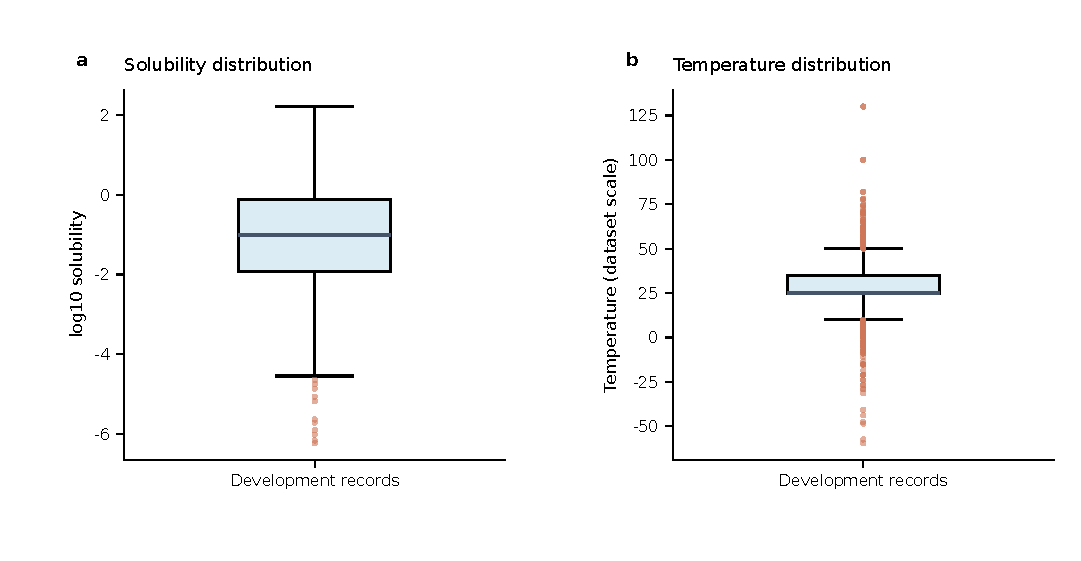
\includegraphics[width=\linewidth]{revision_v2/v2_outliers.pdf}
\caption{开发集极端值识别。箱体表示四分位区间，中线为中位数，须延伸至$1.5\,\mathrm{IQR}$范围内的最远观测，散点表示界限外记录。\textbf{a} 溶解度；\textbf{b} 温度。溶解度的界限外观测集中在低值端，温度的界限外观测分布于两端，反映两类变量不同的尾部结构。}\label{fig:v2outliers}
\end{figure}

\subsection{分子表示与药物母体分组}
每个分子提取11项描述符：分子量、MolLogP、拓扑极性表面积、氢键供体数、氢键受体数、可旋转键数、环数、芳香环数、重原子数、$sp^3$碳比例和形式电荷。药物与溶剂各提供11维，加入温度形成23维基础输入。对于需要标准化的模型，变换仅在训练折内拟合；本文提出模型采用
\begin{equation}
\tilde x_{ij}=\frac{x_{ij}-\mu_j^{(\mathrm{tr})}}{\sigma_j^{(\mathrm{tr})}},
\end{equation}
零方差维度的尺度取1。结构相似度分析另采用半径2、长度1024的Morgan指纹，以Tanimoto系数描述验证药物与训练结构的接近程度。

用于划分的母体键先通过RDKit的ChargeParent获得母体，再移除立体标记，共形成161组。该键将部分盐形式和立体变体归入同组，模型仍读取原始完整分子。数据划分包括1507条开发记录、128个母体，以及397条固定评价记录、33个母体。

\subsection{分布、覆盖与建模启示}
在168$\times$49种可能的结构组合中，仅646种有观测，覆盖率为7.85\%。222种重复组合包含1480条记录，占总数据的77.73\%。重复组合提供条件变化信息，而稀疏的组合覆盖使跨药物推广依赖于结构关系的学习。

温度范围为$-59.5$至130，中位数为25；目标范围为$-6.2343$至$2.2168$。图\ref{fig:v2data}展示结构覆盖、开发目标分布、条件分布和母体记录量。记录集中在少数母体与常见温度，逐行误差因而容易受到高频药物影响。本文将母体等权风险用于训练和评价，使低频药物同样影响总体目标。

\begin{figure}[htbp]\centering
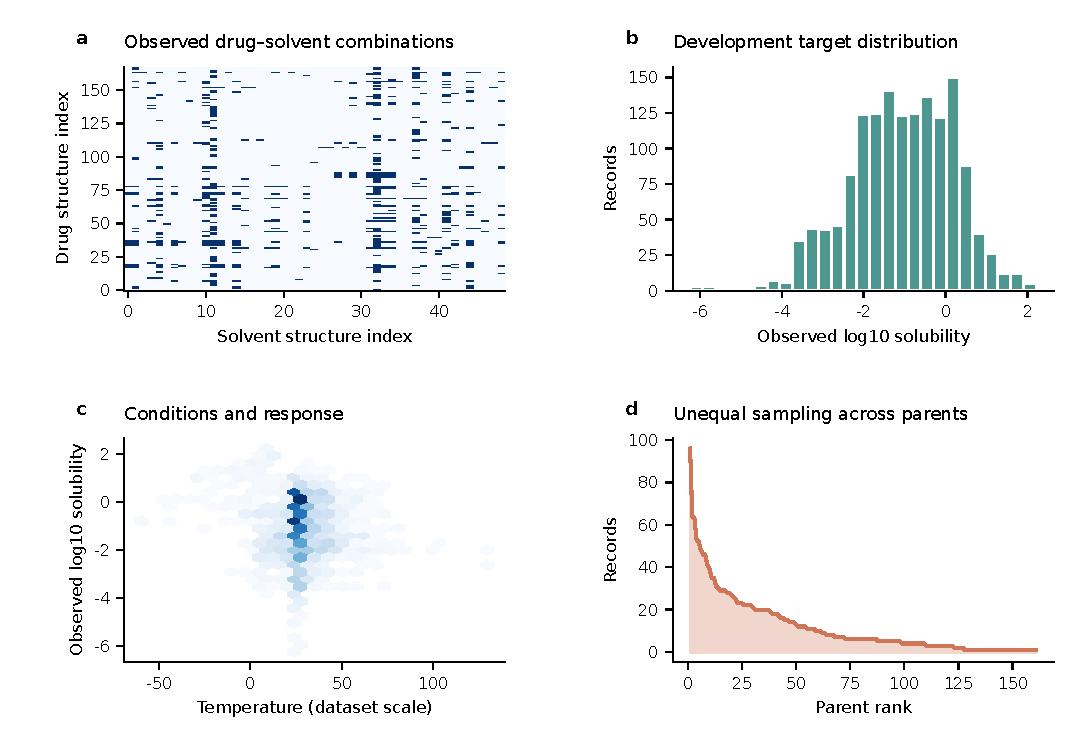
\includegraphics[width=\linewidth]{revision_v2/v2_data.pdf}
\caption{数据结构与探索性分析。\textbf{a} 全部1904条记录的结构组合覆盖，每个单元表示某药物与溶剂组合是否出现。\textbf{b,c} 1507条开发记录的目标分布及温度--目标分布，六边形颜色表示观测密度。\textbf{d} 161个母体按记录数降序排列的采样分布。组合覆盖稀疏且母体记录量差异明显，说明逐行样本量不能替代独立药物覆盖，支持采用母体均衡评价。}
\label{fig:v2data}\end{figure}

同一组合的温度序列则提供了结构间比较无法替代的信息。开发集中，157种组合具有温度变化，对应1118条记录和73个母体。对于同一组合，分子描述符保持不变，两次观测之差主要表达条件变化与实验差异。这些序列为从结构差异中分离温度响应提供了训练信息。


描述符关联进一步揭示了结构与条件信息的不同作用。开发记录中，药物氢键受体数、极性表面积和分子量与目标的Spearman相关系数分别为$-0.496$、$-0.465$和$-0.452$，温度的整体系数为$-0.025$。图\ref{fig:v2associations}给出描述符间关系及药物描述符与目标的关联。结构描述符与目标的关联强于总体温度关联，因而需要进一步在组合内部考察条件响应。

\begin{figure}[htbp]\centering
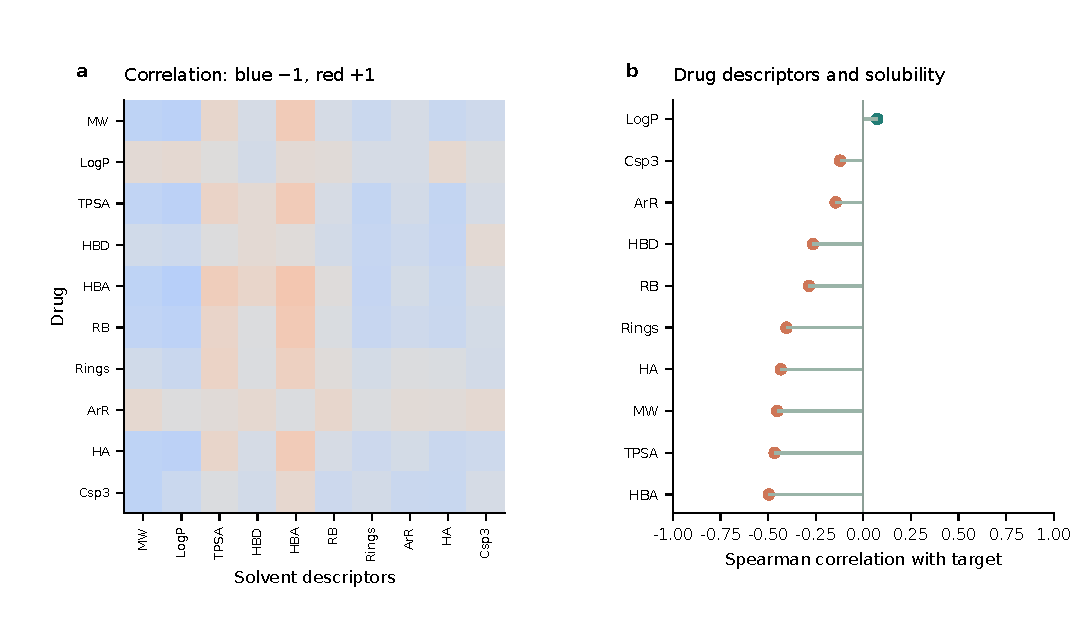
\includegraphics[width=\linewidth]{revision_v2/v2_associations.pdf}
\caption{开发集描述符关联。\textbf{a} 药物与溶剂描述符的Spearman相关矩阵，蓝色对应负相关，红色对应正相关，色阶固定为$[-1,1]$。\textbf{b} 药物描述符与溶解度的相关系数。MW为分子量，RB为可旋转键数，Rings为环数，ArR为芳香环数，HA为重原子数，Csp3为$sp^3$碳比例。药物极性及氢键相关描述符与目标的关联较强，提示结构基线是当前预测任务的重要信息来源。}
\label{fig:v2associations}\end{figure}

如图\ref{fig:v2samplingflow}所示，桑基图按照每个母体的记录数将数据分为1--5条、6--20条和超过20条三层，再连接到开发集与固定评价集。超过20条记录的高频层仅含30个母体，却贡献1078条记录；1--5条记录的低频层包含74个母体，仅贡献182条记录。两层在记录数与母体数上的反差，说明逐行训练会压低大量低频药物的相对贡献。
\begin{figure}[htbp]\centering
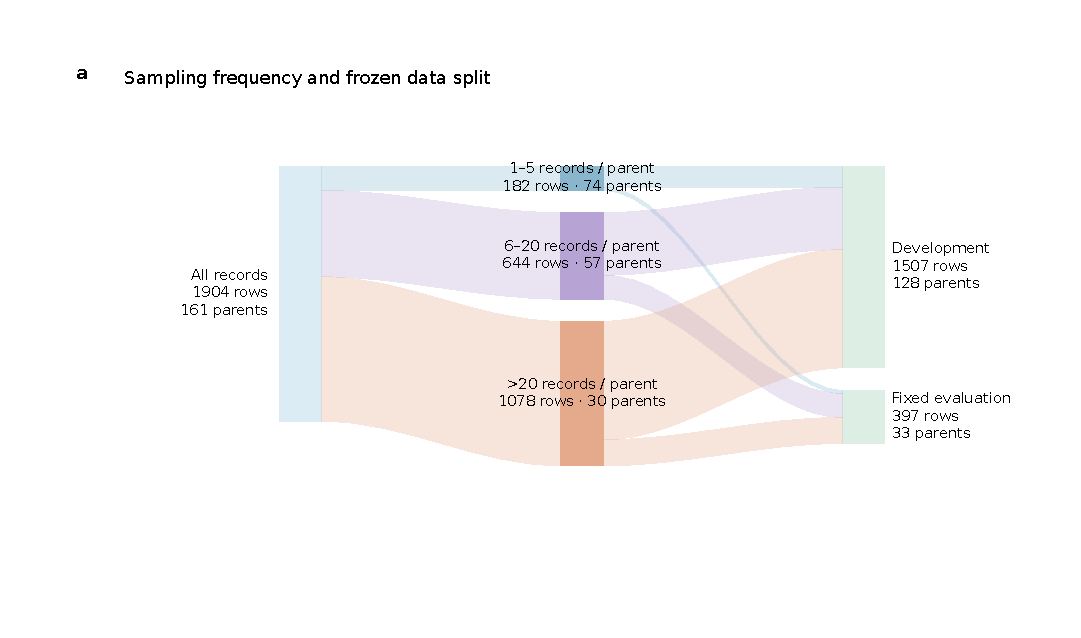
\includegraphics[width=\linewidth]{revision_v2/v2_sampling_flow.pdf}
\caption{采样频次与数据划分桑基图。中间节点依据全量数据的母体记录数分层；流带宽度与记录数成正比，节点标注记录数与独立母体数。高频层的30个母体贡献1078条记录，直观显示记录数量集中于少数药物母体。}\label{fig:v2samplingflow}
\end{figure}

上述分析确定了三个建模环节：按母体均衡训练贡献，以药物--溶剂交互表达组合关系，并从组合内变化学习温度响应。下一章将这些环节写入统一预测分解，再通过增益选择控制温度信息的迁移强度。
